\documentclass[t,11pt]{beamer}

\usepackage{xcolor}
\definecolor{lightgrey}{rgb}{0.9,0.9,0.9}
\definecolor{darkgreen}{rgb}{0,0.6,0}


\usepackage{tipa}

\usepackage{listings}
\lstnewenvironment{latexCode}{%
  \lstset{%
    language=[latex]tex,
    texcsstyle=*\bf\color{blue},
    numbers=none,
    breaklines=true,
    keywordstyle=\color{darkgreen},
    commentstyle=\color{red},
    % otherkeywords={$, \{, \}, \[, \]},
    % frame=none,
    % tabsize=2,
    backgroundcolor=\color{lightgrey},
    % caption=LaTeX example
  }%
}{}



\usetheme[
pagecounter=true,
pageofpages=of,  % page 7 "of" 9
bullet=circle,
titleline=true,
alternativetitlepage=true,
titlepagelogo=images/oxford_big_square,
% titlepagefooterlogo=images/oxford_small_square,
ordinarypageslogo=images/oxford_small_square,
% watermark=images/oxford_small_square,   % bottom right corner
% watermarkheight=100pt,
% watermarkheightmult=4,
]{Torino}
\usecolortheme{greenandblue}
\usefonttheme{structurebold}


\newcommand{\cmd}[1]{\textcolor{blue}{\texttt{#1}}}


\author{Volker Braun}
\title{Git and the New Sage Development Workflow}
\subtitle{Making distributed version control work for you}
\institute{Oxford University}
\date{September 23, 2013}

\begin{document}


\begin{frame}[plain]
	\titlepage
\end{frame}

\begin{frame}{Outline}
	\tableofcontents
\end{frame}



\subsection{Introduction}

\begin{frame}[fragile]
  \frametitle{Linguistic Approach}
  \vspace{-5mm}
  
  \begin{block}{}
    git \textipa{/gIt/}\\
    \textit{v Appalachian \& southern US}\\
    \hspace{1cm} variant of \emph{get}\\
    \textit{n Brit slang pejorative}\\
    \hspace{1cm} foolish or worthless person
  \end{block}
  \bigskip
  \pause

  \small
\begin{verbatim}
GIT(1)                   Git Manual                   GIT(1)

NAME
       git - the stupid content tracker

SYNOPSIS
       git [--version] [--help] [-c <name>=<value>]
           [--exec-path[=<path>]] [--html-path] [--man-path]
           ...
\end{verbatim}

\end{frame}


\begin{frame}
  \frametitle{Git, the DVCS}

  \begin{itemize}
  \item 
    Developed in 2005 to manage the Linux source code
    \begin{quote}
      I'm an egotistical bastard, and I name all my projects after
      myself. First ``Linux'', now ``git'' -- Linus Torvalds
    \end{quote}
  \item Slated to overtake \emph{Subversion} as the most popular VCS
    this year.
  \item \textbf{D}istributed -- there is no central server
  \item \textbf{V}ersion \textbf{C}ontrol \textbf{S}ystem -- manage
    changes to documents
  \item Git is free and open: \url{http://git-scm.com}
  \item Official \texttt{git} implementation: command-line program
  \item Various graphical user interfaces; I like \cmd{gitg} and \cmd{git-cola}
  \item Various websites offer git hosting (Github, Bitbucket,
    Mathematical Institute \url{https://git.maths.ox.ac.uk})
  \end{itemize}

\end{frame}



\begin{frame}
  \frametitle{Demo}
  
  Introduce the following commands:
  \begin{itemize}
  \item 
    Copy repository from github:\\
    \cmd{git clone}
    \\\hfill
    \cmd{https://github.com/vbraun/talk-git-sage-workflow.git}
  \item View history:\\
    \cmd{git log}
  \item Show current branch:\\
    \cmd{git branch}
  \item Switching between branches:\\
    \cmd{git checkout master}\\\cmd{git checkout my\_branch}
  \end{itemize}
\end{frame}



%%% Local Variables:
%%% TeX-master: "talk.tex"
%%% eval: (TeX-PDF-mode 1)
%%% End:


\subsection{Basic Git Concepts}


\begin{frame}
  \frametitle{The Git Directed Acyclic Graph}

  Whenever you run \cmd{git commit}, a snapshot of the current
  state\footnote{Of the \emph{staging} directory tree, see next
    slide.} is added to the repository.
  \begin{itemize}
  \item<2-> Only forward: you can add commits, but never remove them.
  \item<3-> But: you can abandon them.
  \item<4-> Most of the time, commits have one (direct) parent commit and
    one child commit.
  \item<5-> Multiple parents: \emph{Merge} commit
  \item<6-> Multiple children: number can always increase in the future...
  \end{itemize}
\end{frame}


{
  \usebackgroundtemplate{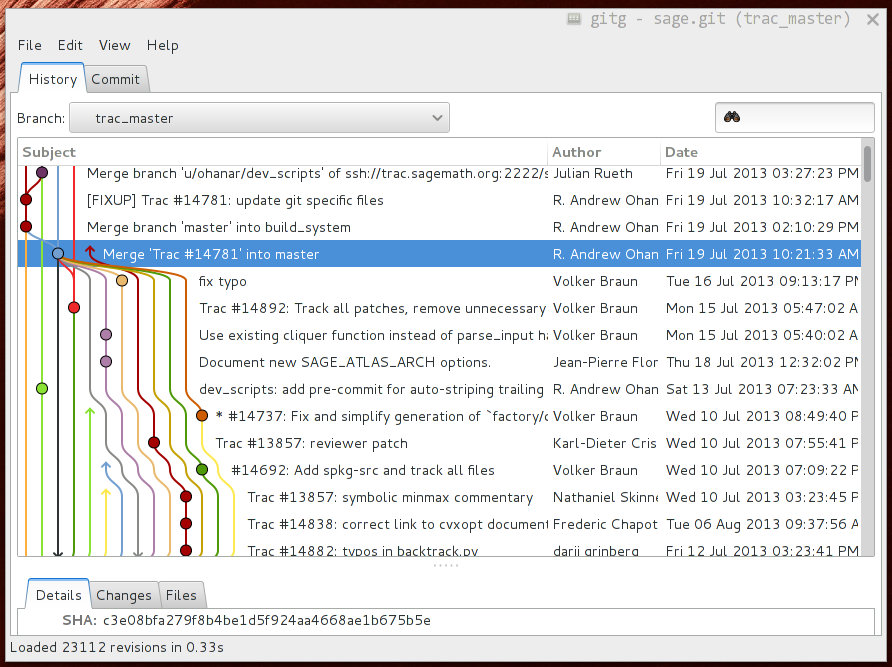
\includegraphics[width=\paperwidth]{images/gitg_screenshot}}
  \begin{frame}[plain]
    % 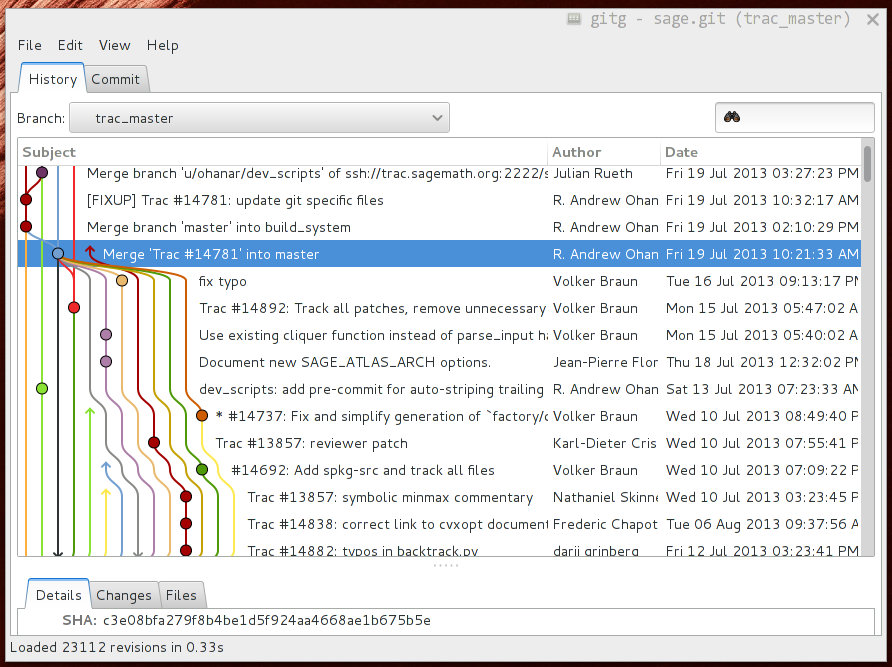
\includegraphics{images/gitg_screenshot}
  \end{frame}
}


\begin{frame}
  \frametitle{The Staging Area}

  Three places to store files:
  \begin{itemize}
  \item<2-> The git database (the \texttt{.git} directory)
  \item<3-> Staging area
  \item<4-> The working directory: all files outside of \texttt{.git} 
  \end{itemize}
  
  \onslide<5->{
    \begin{block}{Staging area}
      The staging area are the files that will be committed by
      \cmd{git commit}
      \begin{itemize}
      \item Show staging: \cmd{git status}
      \item Add to staging: \cmd{git add <filename>}
      \item Remove from staging: \cmd{git reset HEAD <filename>}
      \end{itemize}
    \end{block}
  }
\end{frame}




\begin{frame}
  \frametitle{Committing Changes}

  \begin{block}{Creating a commit}
    \begin{itemize}
    \item 
      \cmd{git commit}
    \item Specify commit message on the command line:\\
      \cmd{git commit -m "my commit message"}
    \end{itemize}
  \end{block}
  
  \onslide<2->{
    Each commit is uniquely specified by the SHA1 hash\footnote{a 40
      digit hex number} of
  }
  \begin{itemize}
  \item<2-> All changes to files
  \item<3-> All parent commits
  \item<4-> The commit message
  \end{itemize}
  \onslide<5->{
    None of these can ever be changed, including all direct and indirect
    parents.
  }
\end{frame}


\begin{frame}
  \frametitle{Branches}

  Branches organize parallel development
  \begin{itemize}
  \item<2-> A branch is just a shortcut for a particular commit
  \item<3-> If you create a new commit, the branch automatically advances
    to it
  \item<4-> The default branch is \texttt{master}, but you can use any name
  \item<5-> \texttt{HEAD} is the commit at the tip of the branch:\\
    \cmd{git show HEAD}
  \item<6-> \texttt{HEAD$\sim$} is the parent of \texttt{HEAD}
  \item<7-> \texttt{HEAD$\sim$2} is the parent of the parent of
    \texttt{HEAD}
  \item<7-> etc.
  \end{itemize}
\end{frame}


\begin{frame}
  \frametitle{Remote Repositories}
  
  \begin{itemize}
  \item<1-> Remotes repositories are bookmarks.
  \item<2-> Configure with \cmd{git remote}
  \item<3-> \textbf{D}istributed VCS: all remotes are equal.
  \item<4-> The "important" one (to you) is usually called \texttt{origin}
  \end{itemize}

  \onslide<5->{
    If there are no conflicts:
  }
  \begin{itemize}
  \item<5-> Upload your changes to the remote repository:\\
    \cmd{git push <remote>}
  \item<6-> Download changes from the remote repository and update the
    local working directory:\\
    \cmd{git pull <remote>}
  \item<7-> There is a default remote for each branch, see\\
    \cmd{git remote show <remote>}
  \end{itemize}

\end{frame}






%%% Local Variables:
%%% TeX-master: "talk"
%%% eval: (TeX-PDF-mode 1)
%%% End:


\section{Conflict Resolution}


\begin{frame}[fragile]
  \frametitle{Merge Conflicts}
  
  \begin{center}
    \Large Don't Panic!
  \end{center}

  \begin{itemize}
  \item 
    Merge conflicts happen if there are overlapping edits.
  \item 
    Resolving them is common and easy.
  \end{itemize}
  
  Example:
  \begin{latexCode}
    \begin{equation}
      \label{eq:quad}
      x = \frac{-b+-\sqrt{b^2-4ac}}{2a}
    \end{equation}
    are the two roots of the quadratic equation.
  \end{latexCode}
  
\end{frame}



\begin{frame}[fragile]
  
  On the flight to a conference I change this to
  \begin{latexCode}
    \begin{equation}
      \label{eq:quad}
      x_{1,2} = \frac{-b+-\sqrt{b^2-4ac}}{2a}
    \end{equation}
    are the two roots of the quadratic equation.
  \end{latexCode}
  \medskip
  \pause
  
  Meanwhile, Jennifer corrects
  \begin{latexCode}
    \begin{equation}
      \label{eq:quad}
      x = \frac{-b\pm\sqrt{b^2-4ac}}{2a}
    \end{equation}
    are the two roots of the quadratic equation.
  \end{latexCode}
  and pushes it to our common remote repository.
  
\end{frame}




%%% Local Variables:
%%% TeX-master: "talk"
%%% eval: (TeX-PDF-mode 1)
%%% End:


\section{Summary}

\begin{frame}[plain]
  \frametitle{Git Operations}
  \centering
  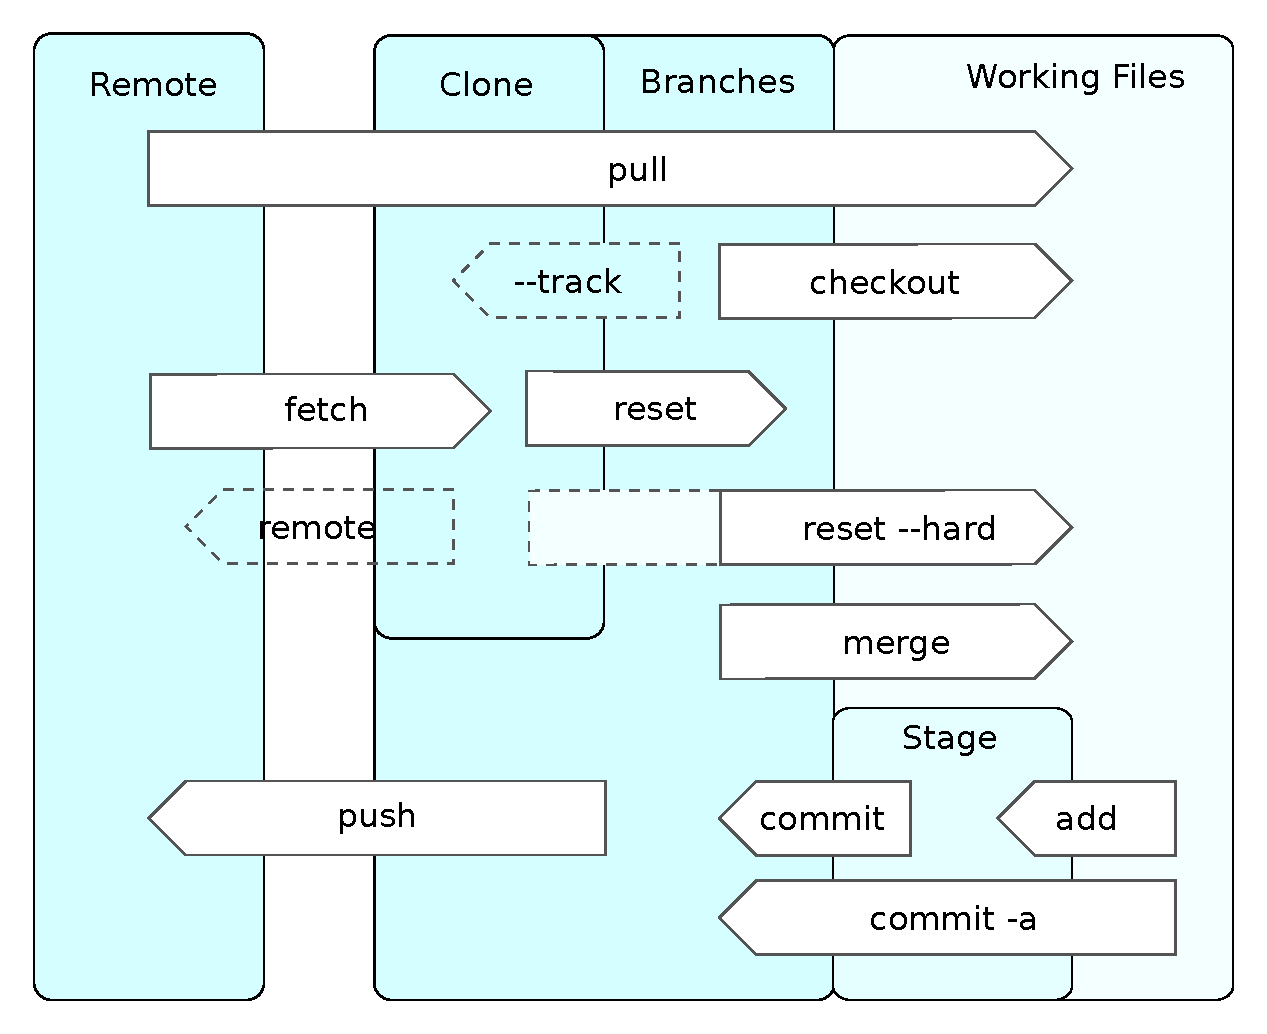
\includegraphics[width=0.85\linewidth]{images/git_operations}
\end{frame}




\end{document}


%%% Local Variables:
%%% eval: (TeX-PDF-mode 1)
%%% End:
